\documentclass{eh-homework}

\usetikzlibrary{arrows.meta}

\begin{document}
    \begin{question}{1}
        Find the error term for the derivative approximation:
        \[
            f''(x_0) \approx \frac{2f(x_0 - h) - 3f(x_0) + f(x_0 + 2h)}{3h^2}.
        \]
        We write the polynomial expansion for each term on the right:
        \[
            f(x_0 - h) = f(x_0) - f'(x_0)h +f''(x_0)h^2 - \frac{f'''(\xi_1)}{6}h^3
        \]
        \[
            f(x_0) = f(x_0)
        \]
        \[
            f(x_0 + 2h) = f(x_0) + 2f'(x_0)h + 4f''(x_0)h^2 + \frac{4f'''(\xi_2)}{3}h^3
        \]
        Then
        \[
            2f(x_0 - h) - 3f(x_0) + f(x_0 + 2h) = 6f''(x_0)h^2 -\frac{2f'''(\xi_1)}{6}h^3 + \frac{4f'''(\xi_2)}{3}h^3
        \]
        \[
            \frac{2f(x_0 - h) - 3f(x_0) + f(x_0 + 2h)}{3h^2} = 2f''(x_0)h^2 - \frac{1}{9}f'''(\xi _1)h + \frac{4}{9}f'''(x_0)h
        \]
        so the error term is
        \[
            f''(x_0) - \left[2f''(x_0)h^2 + \frac{1}{9}f'''(\xi _1)h - \frac{4}{9}f'''(x_0)h \right] = - f''(x_0)h^2 + \frac{1}{9}f'''(\xi _1)h - \frac{4}{9}f'''(x_0)h
        \]
    \end{question}
    \begin{question}{2}
        Find the error term for the quadrature method, and state its degree of precision.
        \[
            \int _{x_0}^{x_0 + 2h}f(x)\ dx \approx \frac{h}{2}\left[ 3f \left( x_0 + \frac{4}{3}h \right) + f(x_0) \right].
        \]
        We expand the left hand side:
        \begin{align*}
            &\ \int _{x_0}^{x_0 + 2h} f(x)\ dx \\
            &= \int _{x_0}^{x_0 + 2h} f(x_0) + f'(x_0)(x - x_0) + \frac{f''(x_0)}{2}(x - x_0)^2 + \frac{f'''(x_0)}{6}(x - x_0)^3 + \frac{f^{(4)}(\xi_1)}{24}(x - x_0)^4\ dx \\
            &= 2f(x_0)h + 2f'(x_0)h^2 + \frac{4}{3}f''(x_0)h^3 + \frac{2}{3}f'''(x_0)h^4 + \frac{4}{15}f^{(4)}(\xi _1)h^5 \\
        \end{align*}
        Now we expand each term on the right hand side:
        \[
            f \left( x_0 + \frac{4}{3}h \right) = f(x_0) + \frac{4}{3}f'(x_0)h + \frac{8}{9}f''(x_0) + \frac{32}{81}f'''(x_0)h^3 + \frac{32}{243}f^{(4)}(\xi _2)h^4.
        \]
        Thus
        \[
            \frac{h}{2}\left[ 3f \left( x_0 + \frac{4}{3}h \right) + f(x_0) \right] = 2f(x_0)h + 2f'(x_0)h^2 + \frac{4}{3}f''(x_0) + \frac{16}{27}f'''(x_0)h^4 + \frac{16}{81}f^{(4)}(\xi_2)h^5.
        \]
        and the error term is
        \[
            \int _{x_0}^{x_0 + 2h}f(x)\ dx - \frac{h}{2}\left[ 3f \left( x_0 + \frac{4}{3}h \right) + f(x_0) \right] = \frac{2}{27}f'''(x_0)h^4 + \frac{4}{15}f^{(4)}(\xi _1)h^5 - \frac{16}{81}f^{(4)}(\xi _2)h^5.
        \]
        and its degree of precision is 2.
    \end{question}
    \begin{question}{3}
        Consider the integral \(\int _1^7 \cos (x^2)\ dx\)
        \begin{enumerate}[label=(\alph*)]
            \item Use the composite Simpson's rule to approximate the value of this integral using \(n=3\) intervals.
            
            We split the interval \([1,7]\) into the three intervals \([1,3], [3,5],[3,7]\) and approximate the integral on each interval. Using Simpson's rule,
            \begin{align*}
                \int _1^7 \cos (x^2)\ dx &= \int _1^3 \cos (x^2)\ dx + \int _3^5 \cos (x^2)\ dx + \int _5^7 \cos (x^2)\ dx \\
                &\approx \frac{(\cos 1^2 + 4 \cos 2^2 + \cos 3^2) + (\cos 3^2 + 4 \cos 4^2 + \cos 5^2)}{3} \\
                &\ + \frac{\cos 5^2 + 4 \cos 6^2 + \cos 7^2}{3} \\
                &\approx -1.985
            \end{align*}
            \item Determine the number of intervals \(n\) needed to guarantee an error of at most \(10^{-4}\).
            
            Using composite Simpson's rule, the absolute error for using \(n\) intervals is \(\frac{6^5}{180n^4}|f^{(4)}(\xi)|\), for some \(\xi \in (1,7)\). If we calculate the fourth derivative of \(f\), we get
            \[
                f^{(4)}(x) = 48x^2 \sin (x^2)+(16x^4 -12)\cos (x^2)
            \]
            so since \(\xi \in (1,7)\),
            \[
                |f^{(4)}(\xi)| \leq 48 \cdot 7^2 + 16 \cdot 7^4 - 12 = 40756
            \]
            Thus the error bound is \(\frac{6^5 \cdot 40756}{180n^4}\). We solve for \(n\) such that \(\frac{6^5 \cdot 40756}{180n^4} < 10^{-4}\) to get
            \[
                n^4 > \frac{6^5 \cdot 10^4 \cdot 40756}{180} \implies n > \sqrt[4]{\frac{6^5 \cdot 10^4 \cdot 40756}{180}} \approx 364.3
            \]
            Thus we need around 365 intervals to guarantee an error better than \(10^{-4}\).
        \end{enumerate}
    \end{question}
    \begin{question}{4}
        Consider the IVP:
        \[
            2\dot y + y = t^4 + 1,\ y(1) = 2.
        \]
        Apply the second degree Taylor method with \(h = 0.5\) to this ODE to approximate \(y(2)\). Show the details in each step.

        \medskip

        We let \(f(t,y) = \dfrac{t^4 - y + 1}{2}\) and rearrange the ODE to see that
        \[
            \dot y = f(t,y).
        \]
        Set \(t_0 = 1, y_0 = y(1) = 2\). Then
        \[
            y_1 = y_0 + \frac{1}{2} f\left(t_0 + \frac{1}{2}, y_0\right) = 2 + \frac{1}{2} f\left(\frac{3}{2}, 2\right) = 2 + \frac{1}{2}\cdot\frac{65}{32} = \frac{129}{64}.
        \]
        \[
            y_2 = y_1 + \frac{1}{2}f(t_1, y_1) = \frac{129}{64} + \frac{1}{2}f\left(2, \frac{129}{64}\right) = \frac{129}{64} + \frac{64 \cdot 2^4 - 129 + 64}{128}
        \]
        \[
            = \frac{129}{64} + \frac{959}{128} = \frac{1217}{128}
        \]
        Thus
        \[
            y(2) \approx \frac{1217}{128}
        \]
    \end{question}
    \begin{question}{5}
        Derive an ODE solver based on the stencil and corresponding integration formula.

        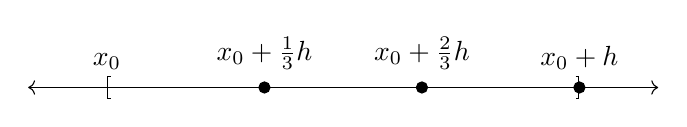
\begin{tikzpicture}
            \draw[<->] (-1, 0) -- (7, 0);
            \draw[{Bracket[width=3mm]}-{Bracket[width=3mm]}] (0, 0) -- (6,0);
            \node[above] at (0, 0.1) {\(x_0\)};
            \foreach \x/\val in {2/\(x_0 + \frac{1}{3}h\), 4/\(x_0 + \frac{2}{3}h\), 6/\(x_0 + h\)} {
                \draw[fill] (\x, 0) circle (2pt);
                \node[above] at (\x, 0.1) {\val};
            }

        \end{tikzpicture}
        Formula: \(\frac{h}{4}\left( 3f \left( x_0 + \frac{1}{3}h \right) + f(x_0 + h) \right) + O (h^4)\)

        \medskip

        Suppose we have the IVT:
        \[
            \dot y = f(t,y),\ y(t_0) = y_0
        \]
        Let \(h = t_{i+1} - t_i\). Define
        \begin{align*}
            k_1 &= f(t_i, y_i) \\
            k_2 &= f \left( t_i + \frac{1}{3}h, y_i + \frac{1}{3}hk_1 \right) \\
            k_3 &= f (t_i + h, y_i + hk_2). \\
        \end{align*}
        Our update step is
        \begin{align*}
            y_{i+1} &= y_i + \int _{t_i}^{t_{i+1}}f(t,y)\ dt \\
            &= y_i + \frac{h}{4}(3k_2 + k_3).
        \end{align*}
    \end{question}
\end{document}